\chapter{Rotårsaksidentifisering}
Arbeidet i denne fasen går ut på å identifisere rotårsaken. I foregående fasen ble en rekke mulige årsaker identifisert og analysert, men nå er det tid for å finne den faktiske rotårsaken. Det er mange forskjellige verktøy som kan brukes i denne fasen, men vi har valgt oss en type årsak-virkning diagram for vårt utgangspunkt.

\section{Årsak-virkningsdiagram}
Et årsak-virkning diagram er et diagram som analyserer forholdene mellom et problem og dets årsaker. Det kombinerer aspekter ved idémyldring med systematisk analyse. Det finnes to typer årsak-virkning diagrammer, fiskebeindiagram og prosessdiagram. Mens et prosessdiagram er mer direkte fokusert på problemet på innsiden av forretningsprosessene, er et fiskebeindiagram en mer generell tilnærming for å adressere alle potensielle årsaker\cite{RCA}. Fiskebeindiagram passer best i dette caset.

\subsection{Ønsket utbytte}
Ved bruk av dette verktøyet ønsker vi å sitte igjen med en visuell fremstilling av rotårsaken til problemet. Dette vil gjøres ved å identifisere hva som skaper årsakene vi har funnet fram til i foregående fase.

\subsection{Gjennomføring}
Det er anbefalt å bruke en tusjtavle for å tegne opp fiskebeindiagrammet, men vi valgte å bruke et nettbasert program som er laget for å skape diagrammer med flere brukere involvert i sanntid. De hadde en egen mal for fiskebeindiagram som vi valgte å gå ut fra. Stegene vi fulgte i prosessen er hentet fra boka om rotårsaksanalyse \cite{RCA} og ble som følger:
\begin{enumerate}
    \item Vi beskrev problemet klart og tydelig
    \item Vi tegnet opp problemet på slutten av fiskebeindiagrammet
    \item Vi identifiserte hovedkategoriene av årsakene til problemet og tegnet det opp på fiskebeinene i diagrammet
    \item Vi idémyldret alle mulige årsaker i hver kategori, en kategori om gangen, og skrev det inn i diagrammet fortløpende
    \item Til slutt analyserte vi de identifiserte årsakene og bestemte de mest sannsynlige rotårsakene
\end{enumerate}

\subsection{Resultater}
Vi beskrev problemet som ulovlig fildeling på skolenettet etter tittelen på caset. Hovedkategoriene vi ønsket å utforske har vi basert på dataanalysen i forrige fase for å finne de mest relevante. Disse var etter vår mening Økonomi, Risiko og Tilgjengelighet. Idémyldringen var i stor grad basert på data og funn fra analysen, med innslag fra den første idémyldringen og andre nye idéer som dukket opp.

\begin{figure}[H]
    \centering
    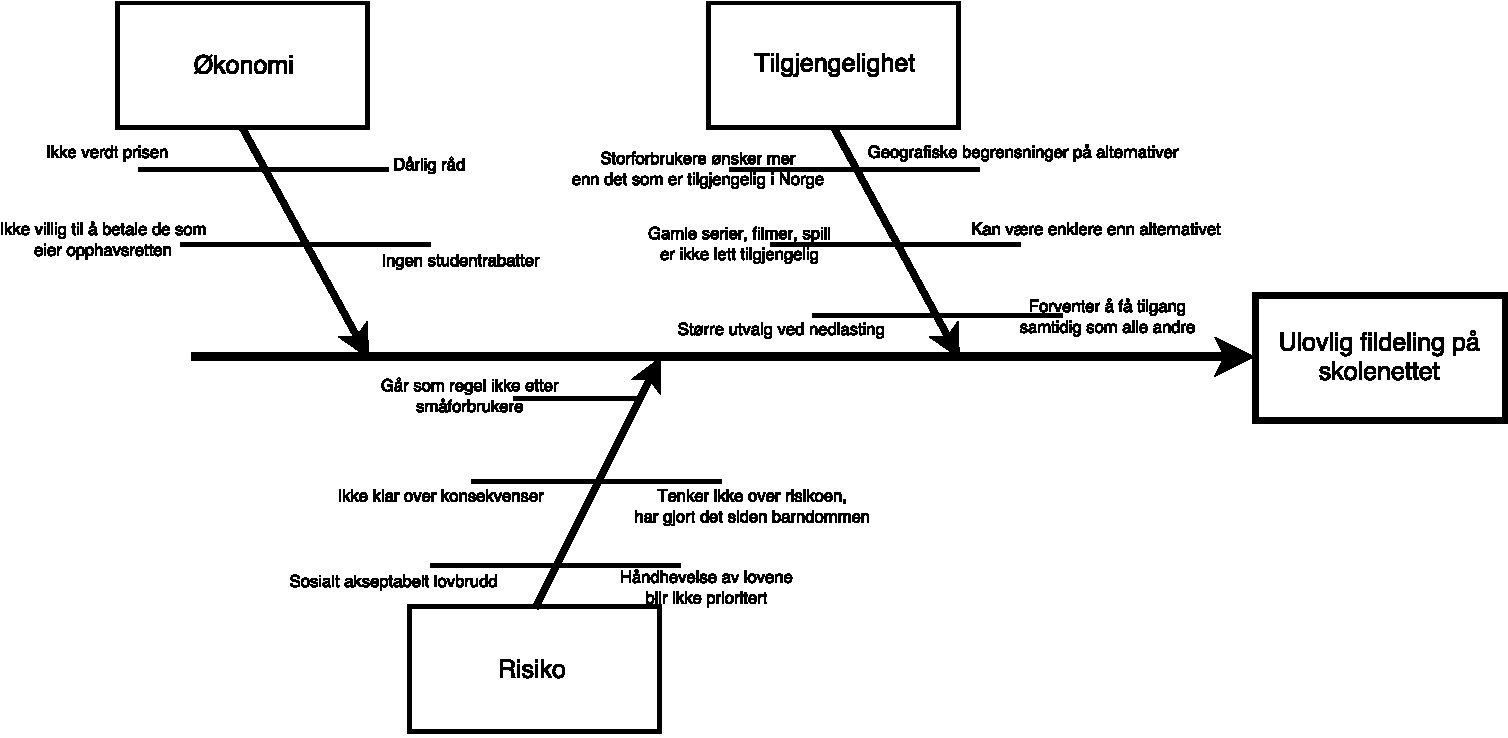
\includegraphics[scale=0.5]{case_1/bilder/fiskebein.pdf}
    \label{fig:fiskebein}
    \caption[Fiskebein]{Fiskebeindiagram over hovedkategorier og årsaker}
\end{figure}

Etter videre analyse av figuren har vi kommet fram til at rotårsaken til fildeling er en kombinasjon flere faktorer, men én skiller seg ut, nemlig tilgjengelighet. Med tilgjengelighet mener vi spesifikt at folk bedriver ulovlig fildeling fordi det er dårligere utvalg på alternative tjenester i Norge. Det finnes også noen mindre årsaker som påvirker folk til å laste ned. Blant dem er at mange føler tjenestene ikke er verdt prisen de må betale når de bare får tilgang på en begrenset mengde materiale. Den siste årsaken går på at håndheving av lovene knyttet til ulovlig fildeling ikke blir prioritert, og derfor har skapt en kultur der det er sosialt akseptabelt å laste ned. Rotårsakene er listet etter viktighet der den første er hovedårsaken:

\begin{enumerate}
    \item Dårligere utvalg på alternative tjenester i Norge
    \item Tjenestene er ikke verdt prisen
    \item Håndheving og kommunisering av lovene knyttet til ulovlig fildeling blir ikke prioritert
\end{enumerate}

\subsection{Konklusjon av verktøy}
Verktøyet fungerte som en strukturert måte å kategorisere alle mulige rotårsaker vi hadde kommet fram til i tidligere faser. Det var også mulighet for å inkludere andre mulige årsaker som vi hadde i tankene gjennom prosessen. Det kan kanskje i noen sammenhenger være vanskelig å kategorisere de ulike årsakene dersom disse gruppene ikke er klart definert på forhånd, men i denne sammenhengen var det veldig intuitivt. Det kan også hende idémyldringen blir litt for fokusert på de ulike kategoriene siden man definerer disse på forhånd. Ellers et veldig godt verktøy som ga oss relevante resultater. 